\section{Auswertung}
\label{sec:Auswertung}
In den folgenden Tabellen sind die gemessenen Werte zusammenfassend dargestellt.

\begin{table}[H]
  \centering
  \caption{Die Messwerte der Reflexion an einem Spiegel für verschiedene Winkel. Verwendet wurde der grüne Laser mit $\lambda = \SI{532}{\nano\meter}$.}
  \label{tab:MessungAufgabe1}
  \sisetup{table-format=2.1}
  \begin{tabular}{S S}
    \toprule
    {Einfallswinkel[\si{\degree}]} & {Ausfallswinkel[\si{\degree}]} \\
    \midrule
    69   &  69   \\
    42   &  43   \\
    30.5 & 30.5  \\
    55   & 56    \\
    72   & 72    \\
    20   & 20    \\
    35   & 35    \\
    52   & 52.5  \\
    \bottomrule
  \end{tabular}
\end{table}

\begin{table}[H]
  \centering
  \caption{Die Messwerte der Brechung an einer planparallelen Platte der Messung 1 für verschiedene Winkel. Verwendet wurde der grüne Laser mit $\lambda = \SI{532}{\nano\meter}$.}
  \label{tab:MessungAufgabe2}
  \sisetup{table-format=2.2}
  \begin{tabular}{S S}
    \toprule
    {Einfallswinkel[\si{\degree}]} & {Brechungswinkel[\si{\degree}]} \\
    \midrule
    69 & 39    \\
     0 &  0    \\
    10 &  7    \\
    30 & 20    \\
    40 & 25.5  \\
    75 & 40.5  \\
    55 & 33.5  \\
    38 & 24.25 \\
    \bottomrule
  \end{tabular}
\end{table}

\begin{table}[H]
  \centering
  \caption{Die Messwerte der Brechung an einer planparallelen Platte der Messung 2 für verschiedene Winkel. Verwendet wurde der grüne Laser mit $\lambda = \SI{532}{\nano\meter}$.}
  \label{tab:MessungAufgabe3}
  \sisetup{table-format=2.1}
  \begin{tabular}{S S}
    \toprule
    {Einfallswinkel[\si{\degree}]} & {Brechungswinkel[\si{\degree}]} \\
    \midrule
    0  &  0     \\
   45  & 28.5   \\
   60  & 36     \\
   20  & 13.5   \\
   51  & 31.5   \\
    3  &  3.5   \\
    \bottomrule
  \end{tabular}
\end{table}

\begin{table}[H]
  \centering
  \caption{Die Messwerte der Brechung an einem Prisma für verschiedene Winkel. Verwendet wurde der grüne Laser mit $\lambda = \SI{532}{\nano\meter}$ und der rote Laser mit $\lambda = \SI{635}{\nano\meter}$.}
  \label{tab:MessungAufgabe4}
  \sisetup{table-format=2.1}
  \begin{tabular}{S S S}
    \toprule
    {Einfallswinkel[\si{\degree}]} & {Ausfallswinkel $L_{Gruen}$[\si{\degree}]} & {Ausfallswinkel $L_{Rot}$[\si{\degree}]} \\
    \midrule
    30  & 82   & 84   \\
    35  & 73.5 & 74.5 \\
    39  & 60   & 60.7 \\
    46  & 48   & 49.5 \\
    60  & 42   & 43   \\
    \bottomrule
  \end{tabular}
\end{table}

\begin{table}[H]
  \centering
  \caption{Die gemessenen Beugungsmaxima der Beugung an einem Strichgitter mit 600 Linien/mm. Verwendet wurde der grüne Laser mit $\lambda = \SI{532}{\nano\meter}$.}
  \label{tab:MessungAufgabe51}
  \sisetup{table-format=2.1}
  \begin{tabular}{S S S }
    \toprule
    {Laserposition[\si{\degree}]} & $B_{max1,2}$[\si{\degree}] & $B_{max3}$[\si{\degree}]\\
    \midrule
    0  & \pm 22.5 & 0 \\
    \bottomrule
  \end{tabular}
\end{table}

\begin{table}[H]
  \centering
  \caption{Die gemessenen Beugungsmaxima der Beugung an einem Strichgitter mit 300 Linien/mm.}
  \label{tab:MessungAufgabe52}
  \sisetup{table-format=2.1}
  \begin{tabular}{S S S S}
    \toprule
    {Laserposition[\si{\degree}]} & $B_{max1,2}$[\si{\degree}] & $B_{max3,4}$[\si{\degree}] & $B_{max5}$[\si{\degree}]\\
    \midrule
    0 & \pm 22 & \pm 10.7 & 0 \\
    \bottomrule
  \end{tabular}
\end{table}

\begin{table}[H]
  \centering
  \caption{Die gemessenen Beugungsmaxima der Beugung an einem Strichgitter mit 100 Linien/mm.}
  \label{tab:MessungAufgabe53}
  \sisetup{table-format=2.1}
  \begin{tabular}{S S S S S S S S S}
    \toprule
    {Laserposition[\si{\degree}]} & $B_{1,2}$[\si{\degree}] & $B_{3,4}$[\si{\degree}] & $B_{5,6}$[\si{\degree}] & $B_{7,8}$[\si{\degree}] & $B_{9,10}$[\si{\degree}] & $B_{11,12}$[\si{\degree}]  & $B_{13,14}$[\si{\degree}] & $B_{15}$[\si{\degree}]\\
    \midrule
    0 & \pm 26 & \pm 22 & \pm 18 & \pm 14 & \pm 11 & \pm 7.2 & \pm 3.7 & 0 \\
    \bottomrule
  \end{tabular}
\end{table}

\subsection{Reflexion}
\label{sec:reflexionauswertung}
Die Ergebnisse der Untersuchung der Reflexion sind in Tabelle \ref{tab:MessungAufgabe1} abgebildet. Die maximale Genauigkeit der Messung liegt ungefähr bei einem Grad, da die Skalen, von denen abgelesen wurden, keine kleineren Unterteilungen besaßen. Nach dem Reflexionsgesetz
\eqref{eqn:reflexion} beträgt die maximale Abweichung der Messung von der Theorie $\pm \SI{1}{\degree}$.
Im der folgenden Abbildung sind der Einfallswinkel und der Reflexionswinkel gegeneinander aufgetragen.

\begin{figure}
  \centering
  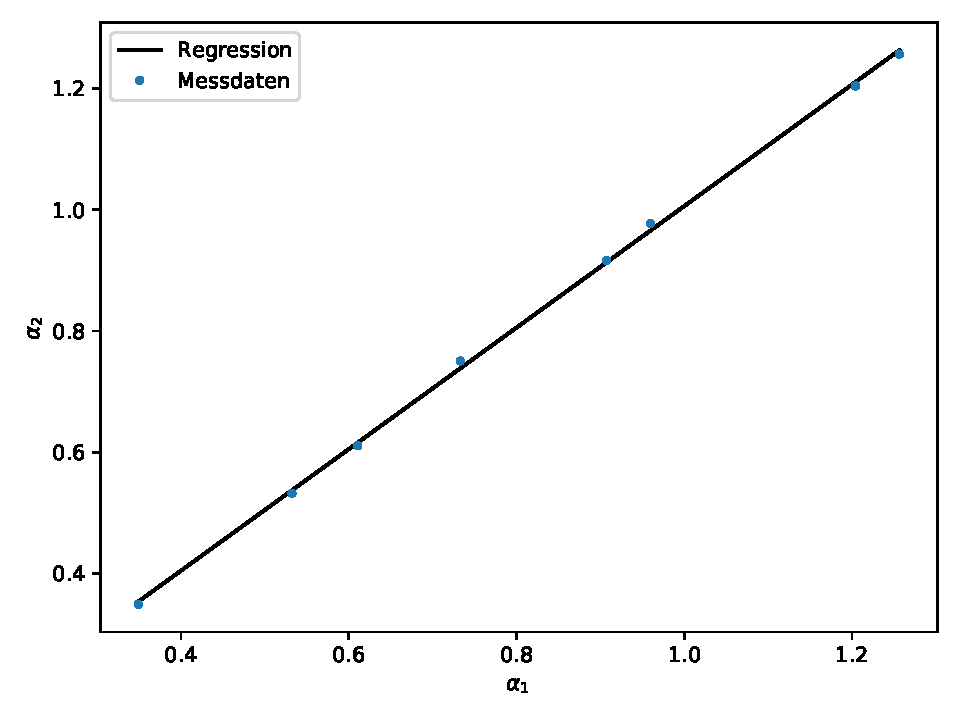
\includegraphics[scale= 0.7]{auswertung/plot1.pdf}
  \caption{Einfallswinkel $\alpha_1$ und Reflexionswinkel $\alpha_2$ gegeneinander aufgetragen.}
  \label{fig:plot1}
\end{figure}

\subsection{Brechung}
\label{sec:brechungauswertung}
Die bestimmten Brechungswinkel sind in Tabelle \ref{tab.Aufgabe2} abgebildet.
Der Brechungsindex berechnet nach dem Brechungsgesetz \eqref{eqn:brechung2} mit den gemessenen Daten beträgt
\begin{equation}
  n = 0.010 \pm 0.010.
  \label{eqn:brechungsindexausw}
\end{equation}
Die Literaturwerte für den Brechnungsindex sind in Tabelle \ref{tab:brechungsind} angegeben.


\subsection{Planparalle Platten}
\label{sec:planplatteauswertung}
\subsection{Prisma}
\label{sec:prismaauswertung}
\subsection{Beugung am Gitter}
\label{sec:beugungauswertung}
